\chapter{evaluation}

\section{Methodology}

\section{Experimental Configuration}

Evaluation of the Vehicle Actuated control strategy, PBTC control strategy, and SCATS representation was carried out within PBTSim on the two-way intersection configuration described in Section ~\ref{sec:ScenarioDesign}.

% describe the traffic configuration settings
% list of metrics and explanation


\begin{figure}
\centering
\begin{subfigure}{.5\textwidth}
  \centering
  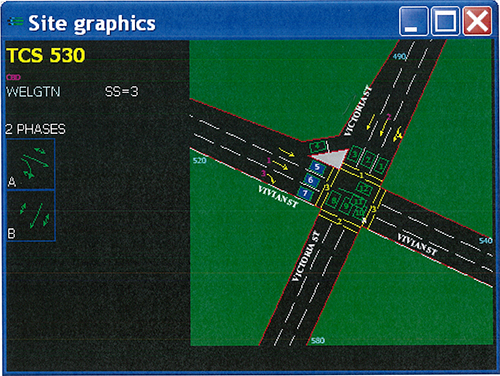
\includegraphics[scale=0.35]{scats-vivian-victoria.png}
  \caption{A subfigure}
  \label{fig:sub1}
\end{subfigure}%
\begin{subfigure}{.5\textwidth}
  \centering
  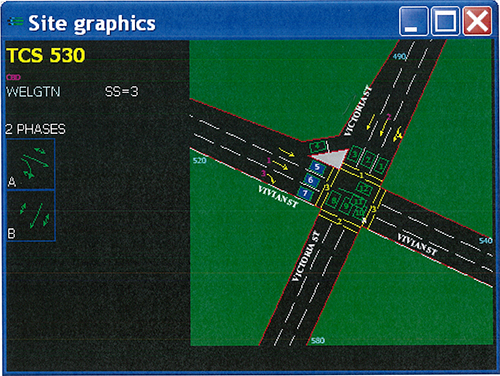
\includegraphics[scale=0.35]{scats-vivian-victoria.png}
  \caption{A subfigure}
  \label{fig:sub2}
\end{subfigure}

\vspace{1cm}

\begin{subfigure}{.5\textwidth}
  \centering
  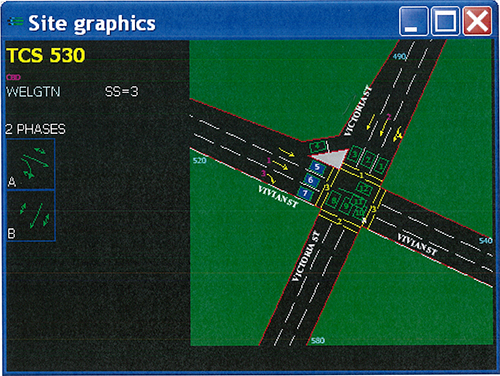
\includegraphics[scale=0.35]{scats-vivian-victoria.png}
  \caption{A subfigure}
  \label{fig:sub1}
\end{subfigure}%
\begin{subfigure}{.5\textwidth}
  \centering
  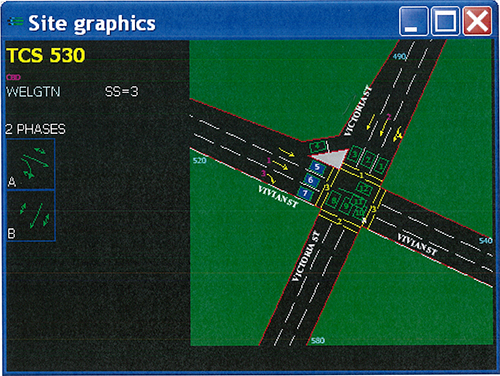
\includegraphics[scale=0.35]{scats-vivian-victoria.png}
  \caption{A subfigure}
  \label{fig:sub2}
\end{subfigure}
\caption{The intersection of Vivian Street and Victoria Street in Te Aro, Wellington City, as viewed in the SCATS management application in use by Wellington City Council. }
\label{fig:test}
\end{figure}
